\documentclass[conference,letterpaper]{IEEEtran}
\usepackage[T1]{fontenc}
\usepackage[utf8]{inputenc}
\usepackage{graphicx}
\usepackage{url}
\renewcommand{\abstractname}{Resumen}
\renewcommand{\IEEEkeywordsname}{Palabras clave}
\renewcommand{\refname}{Referencias}

\title{Sistema web ERP y punto de venta para Restaurante Orígenes SV}
\author{\IEEEauthorblockN{Amy Ariadna Barraza Villacorta, Andrés Eduardo Vega Mena, Johann André Angel Menjívar,\\
Rodrigo Josué Medrano Márquez, Magaly Brendalí Aguilar Granillo, Alfredo Antonio Guarita Hernández,\\
Daniel Alexander Avelar Orellana y Saul Ernesto Giron Vigil}
\IEEEauthorblockA{Equipo Nexo Bytecode, Programación Web, Universidad Centroamericana José Simeón Cañas\\
El Salvador, ciclo 02 de 2026}}

\begin{document}
\maketitle

\begin{abstract}
Restaurante Orígenes SV requiere coordinar ventas, existencias, compras, caja y nómina entre sucursales. Se desarrolló una aplicación web que relaciona el punto de venta con recetas, movimientos de inventario y turnos de caja. Este artículo presenta la arquitectura, el modelo de datos y las reglas de negocio, y valida el flujo con PostgreSQL 18 en una base inicializada con el seed principal. Se registraron comprobantes CF y CCF de Latte Grande, se verificó el consumo de cinco insumos, se registró una compra a crédito, se obtuvo un cierre sin diferencias y se generó una planilla quincenal para ocho empleados de demostración.
\end{abstract}

\begin{IEEEkeywords}
ERP, punto de venta, inventario por sucursal, transacciones, nómina.
\end{IEEEkeywords}

\section{Introducción}
El caso de Restaurante Orígenes SV plantea mantener una operación común para varias sucursales \cite{enunciado}. Los operadores necesitan saber qué productos pueden vender con los insumos disponibles; gerencia necesita controlar existencias, facturas de compra, pagos y personal. Registrar estos procesos de forma aislada dificulta relacionar una venta con su turno y con el consumo real de materiales. El objetivo fue implementar un sistema que vincule esas operaciones y permita demostrar la trazabilidad con datos persistentes.

El alcance comprende el catálogo de elaborados y reventa, documentos de consumidor final y crédito fiscal, pagos, recepción de compras, control de caja y planilla. El seed principal prepara tres sucursales, cuatro cuentas por rol, quince elaborados y cuatro productos de reventa. También carga clientes con datos fiscales, proveedores, compras, cuentas por pagar, empleados y tramos de renta.

\section{Arquitectura y modelo de datos}
El cliente React organiza la navegación y presenta formularios y resultados. Vite construye el frontend y Tailwind se usa en la interfaz. El cliente Axios intercambia JSON con una API Express. Los controladores validan las solicitudes y delegan las reglas de negocio en servicios. El JWT transporta la identidad de sesión \cite{jwt}; la aplicación usa el rol y la sucursal para limitar operaciones donde corresponde. La Fig.~\ref{fig:arquitectura} muestra el recorrido de la solicitud.

\begin{figure}[!t]
\centering
\small
\begin{tabular}{c}
\fbox{Operador de sucursal} \\
$\downarrow$ \\
\fbox{React, Vite y Tailwind} \\
$\downarrow$ HTTP, JSON y JWT \\
\fbox{Express: rutas, controladores y servicios} \\
$\downarrow$ consultas y transacciones \\
\fbox{Prisma y PostgreSQL}
\end{tabular}
\caption{Capas de la aplicación y flujo de una solicitud.}
\label{fig:arquitectura}
\end{figure}

El catálogo es común y el stock se identifica por insumo y sucursal. Una receta relaciona un producto elaborado con sus insumos y cantidades por unidad. El producto de reventa referencia directamente el insumo descontado. Cada venta se vincula a un turno, sus líneas y pagos. Cada compra registra sus detalles y puede originar una cuenta por pagar con abonos. Las planillas contienen el detalle de deducciones por empleado. La Fig.~\ref{fig:modelo} resume las relaciones que conectan estos registros.

\begin{figure}[!t]
\centering
\small
\begin{tabular}{l}
Sucursal $\rightarrow$ Turno $\rightarrow$ Venta $\rightarrow$ Pago \\
Venta $\rightarrow$ VentaDetalle $\leftarrow$ Producto \\
Sucursal $\rightarrow$ StockSucursal $\leftarrow$ Insumo \\
Producto $\rightarrow$ RecetaItem $\leftarrow$ Insumo \\
Proveedor $\rightarrow$ Compra $\rightarrow$ CuentaPorPagar \\
CuentaPorPagar $\rightarrow$ Abono \\
Planilla $\rightarrow$ PlanillaDetalle $\leftarrow$ Empleado
\end{tabular}
\caption{Relaciones principales del modelo. Cada flecha conecta una entidad con los registros que la referencian.}
\label{fig:modelo}
\end{figure}

El diseño de las escrituras relacionadas se apoya en la atomicidad de PostgreSQL \cite{postgres} y en las transacciones de Prisma \cite{prisma}. El servicio de ventas asigna un correlativo por sucursal y tipo, descuenta existencias y crea la venta dentro de una transacción. El movimiento de inventario conserva la referencia al comprobante. La compra registra las líneas, la entrada de existencias y su obligación de pago cuando corresponde.

\section{Implementación del caso}
\subsection{Latte Grande y comprobantes}
El Latte Grande del seed cuesta \$3.50 con IVA. Su receta consume 18 g de café, 250 ml de leche entera, un vaso de 16 oz, una tapadera y una viñeta por unidad. El catálogo calcula cuántas unidades puede despachar con el insumo limitante. Al vender dos unidades se descuentan 36 g, 500 ml y dos de cada material de empaque en la sucursal del turno.

El servicio aplica el IVA del 13\,\% en CF y CCF \cite{enunciado}. Para una línea de \$3.50 divide el total entre 1.13 y redondea la base a \$3.10. La diferencia de \$0.40 corresponde al IVA. El usuario puede emitir CF sin cliente fiscal; para CCF debe seleccionar un cliente con NIT y NRC. El historial permite consultar el documento emitido.

\begin{figure}[!t]
\centering
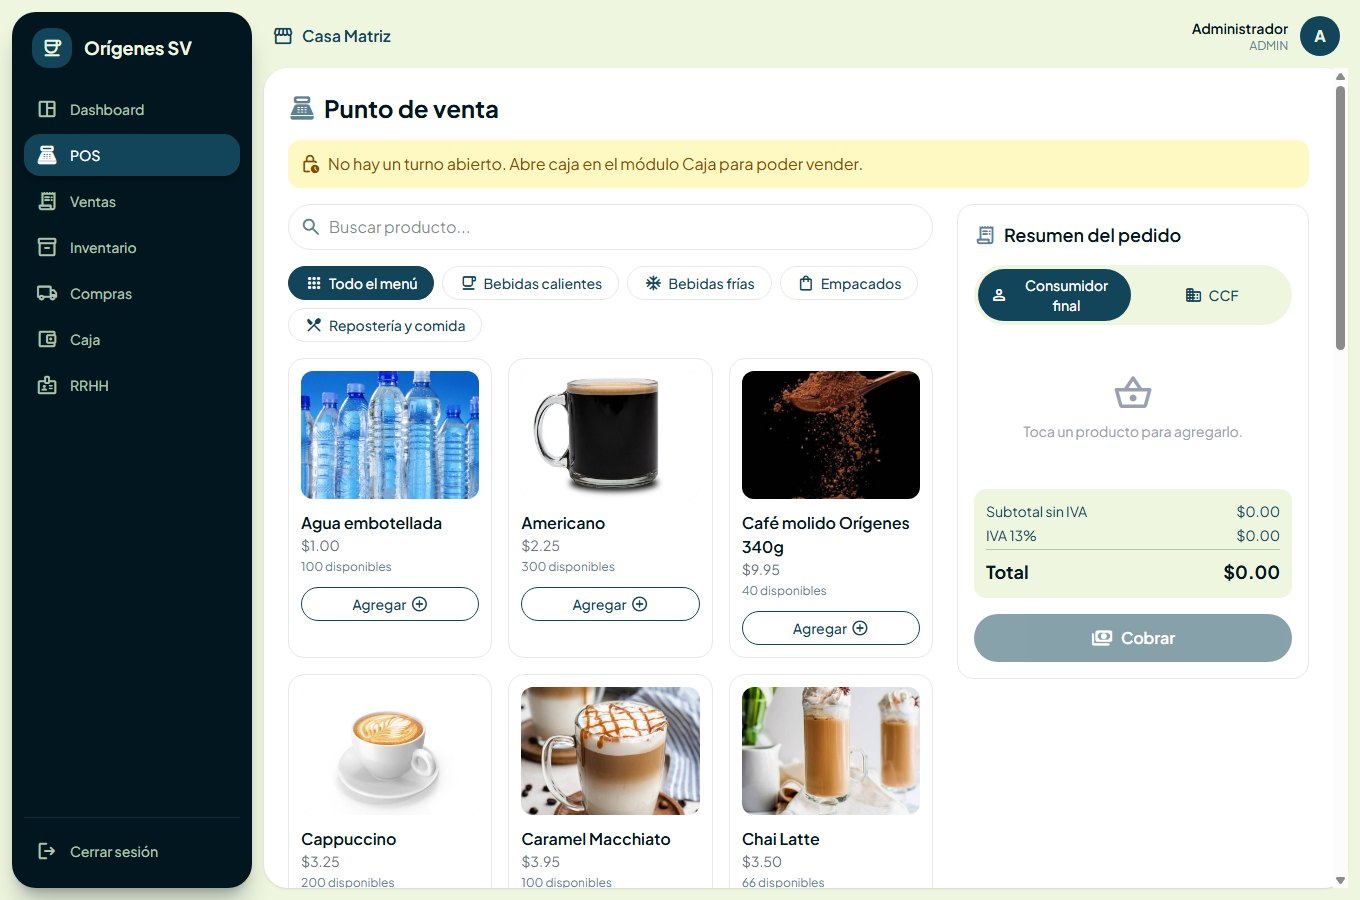
\includegraphics[width=\columnwidth]{../capturas/pos.jpg}
\caption{Catálogo POS en ejecución con los productos del seed.}
\label{fig:pos}
\end{figure}

\subsection{Compras y caja}
El registro de una compra a crédito suma las cantidades de inventario de su sucursal y deja una cuenta por pagar. Los abonos reducen el saldo y modifican el estado. El cierre de turno compara lo esperado con lo contado en efectivo, tarjeta y digital. El efectivo esperado incorpora el fondo inicial y los pagos en efectivo de ventas emitidas del turno. Los pagos con Bitcoin y Chivo Wallet forman el total digital del cuadre.

\subsection{Planilla y retención de renta}
El cálculo parte del salario mensual dividido entre dos. La implementación descuenta ISSS del 3\,\% con un tope de base quincenal de \$500 y AFP del 7.25\,\% sobre el bruto. La base de renta es el bruto menos ambas cotizaciones. Se selecciona el tramo cargado en \texttt{TramoRenta} y se suma su cuota fija al porcentaje sobre el exceso. El Decreto Ejecutivo n.\textsuperscript{o} 10 documenta las tablas de retención \cite{renta}; los valores del seed se usan en el cálculo de la demostración.

Por ejemplo, con \$950 mensuales, el bruto quincenal es \$475.00, ISSS es \$14.25 y AFP es \$34.44. La base de renta es \$426.31. El segundo tramo aporta \$8.83 más el 10\,\% del exceso sobre \$275.00, para una retención redondeada de \$23.96 y un neto de \$402.35.

\begin{figure}[!t]
\centering
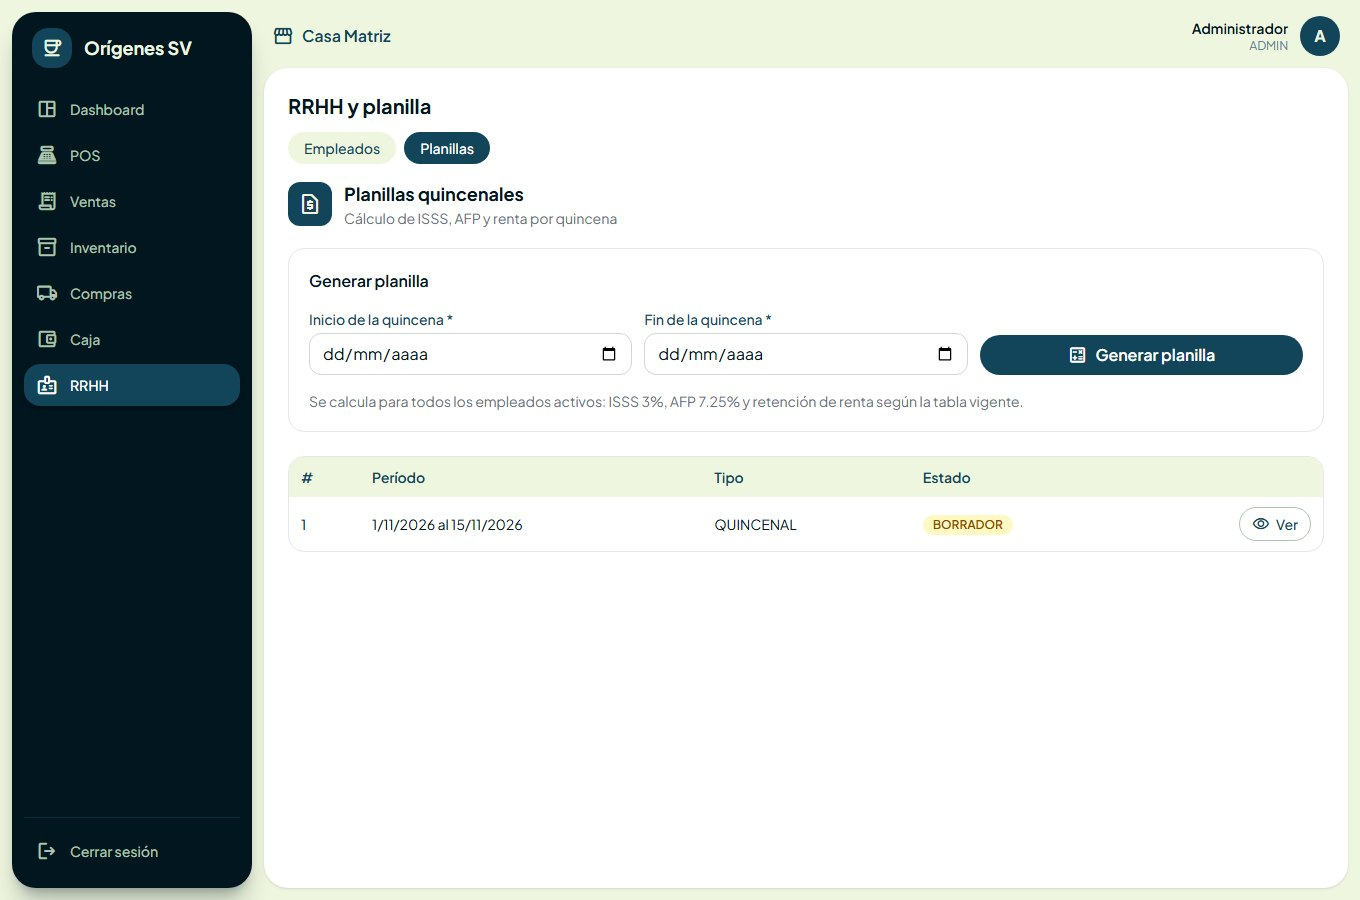
\includegraphics[width=\columnwidth]{../capturas/planillas.jpg}
\caption{Módulo de planillas con el período generado durante la verificación.}
\label{fig:planillas}
\end{figure}

\section{Organización del equipo}
El repositorio usa ramas por módulo y pull requests para integrar en \texttt{develop}. Amy Ariadna Barraza Villacorta trabajó en caja. Andrés Eduardo Vega Mena implementó inventario y recetas. Johann André Angel Menjívar trabajó en compras y datos de demostración. Rodrigo Josué Medrano Márquez desarrolló el POS y elementos comunes de interfaz. Magaly Brendalí Aguilar Granillo trabajó en ventas y comprobantes. Alfredo Antonio Guarita Hernández trabajó en empleados, planilla e integración de pantallas. Daniel Alexander Avelar Orellana preparó QA, documentación y despliegue. Saul Ernesto Giron Vigil trabajó en el esquema inicial, autenticación, frontend base y sucursales. El Excel relaciona actividades, fechas y commits de cada integrante.

\section{Verificación de la implementación}
Se ejecutó la versión integrada \texttt{3575d81} en una copia temporal. Se aplicó la migración versionada a PostgreSQL 18 y se ejecutó el seed principal. La verificación combinó operaciones HTTP con capturas del frontend en ejecución. Las cuatro cuentas iniciaron sesión. Se contrastaron los permisos del POS y de RR. HH. por rol y la devolución de HTTP 401 sin sesión en una ruta protegida, coherente con el uso de ese código para solicitudes sin credenciales válidas \cite{http}.

\begin{table}[!t]
\caption{Resultados sobre la base de demostración}
\label{tab:resultados}
\centering
\footnotesize
\begin{tabular}{@{}p{0.27\columnwidth}p{0.65\columnwidth}@{}}
\hline
Flujo & Evidencia observada \\
\hline
Acceso & Cuatro cuentas, permisos de POS y RR. HH., y tres sucursales. \\
Catálogo & 19 productos disponibles en la consulta del POS. \\
Ventas & CF y CCF de \$3.50 con base \$3.10 e IVA \$0.40. \\
Receta & Dos ventas descontaron los cinco insumos en las cantidades previstas. \\
Compras & Compra a crédito con incremento de 100 g de café y cuenta por pagar. \\
Caja & Fondo inicial \$20.00, ventas \$7.00 y cierre sin diferencias. \\
Planilla & Generación y consulta de ocho detalles del período del 1 al 15 de noviembre. \\
\hline
\end{tabular}
\end{table}

Se consultó el comprobante después de cada venta y se comparó el stock anterior y posterior. El detalle de planilla confirmó las deducciones del ejemplo de \$950 mensuales. La planilla se generó desde el formulario. La interfaz envió el inicio y el fin a mediodía y mostró del 1 al 15 de noviembre en la zona horaria de Guatemala (Fig.~\ref{fig:planillas}). Las pruebas cubrieron la base de demostración. La concurrencia y la carga de producción quedan fuera del alcance de esta ejecución.

\section{Conclusiones}
El sistema vinculó operaciones de venta, inventario y caja en la base de demostración. El Latte Grande permitió contrastar receta, cálculo de IVA, movimientos de existencias y cuadre con una operación concreta. La compra a crédito y la planilla confirmaron que el mismo entorno soporta los flujos administrativos evaluados. La migración versionada y el seed principal permiten repetir la demostración con otra base local.

\section*{Uso de inteligencia artificial}
El equipo declara OpenAI Codex y Anthropic Claude en la bibliografía. Daniel Avelar usó Codex para QA con PostgreSQL, capturas, despliegue local, seguimiento de actividades y preparación de la documentación y del informe IEEE \cite{codex}.

Anthropic Claude apoyó a J. Angel en el módulo de compras y proveedores, tanto en el backend como en el frontend. El apoyo abarcó el registro de compras con entrada de inventario y cuentas por pagar, abonos y estado de cuenta, además del seed de demostración, la consulta de sucursales y el manejo de errores de validación. También apoyó la integración del nuevo inicio de sesión, las imágenes del catálogo POS, el cliente HTTP compartido, el selector de sucursal en empleados, correcciones de lint y rutas, el borrador del README y la revisión del repositorio y de los entregables \cite{claude}. Las funciones \texttt{registrarCompra} y \texttt{registrarAbono} están marcadas en el código fuente. Johann confirmó que revisó los cambios de código y que se integraron por pull request.

A. Vega desarrolló Inventario y Recetas. Definió los requisitos y los contratos con Ventas, Compras y POS, revisó los cambios y los integró por pull request. Claude Code apoyó los formularios controlados y el estado inmutable, la carga en paralelo, el editor dinámico de recetas, el renderizado condicional, las alertas, React Router, Axios y la migración a Tailwind. En el backend asistió en el descuento atómico con \texttt{updateMany} y \texttt{gte}, las transacciones de Prisma, \texttt{upsert}, \texttt{connectOrCreate}, \texttt{disconnect} y la adaptación al stock por sucursal y al kárdex \cite{claude}.

Amy Ariadna Barraza Villacorta usó Claude en Caja para las rutas, la autenticación y los roles, la transacción de cierre y el manejo de estado, montos y fechas. Rodrigo Medrano usó Claude Code en POS para el catálogo, la disponibilidad por receta, la búsqueda de clientes para CCF, el carrito, los pagos mixtos y el vuelto, Axios y el diseño con Tailwind. \cite{claude}.

\IEEEtriggeratref{2}
\begin{thebibliography}{9}
\bibitem{enunciado}
“Proyecto de Cátedra, Programación Web, Ciclo 02, 2026,” enunciado académico, 2026, pp. 1--5.
\bibitem{jwt}
M. Jones, J. Bradley y N. Sakimura, “JSON Web Token (JWT),” RFC 7519, mayo 2015. \url{https://www.rfc-editor.org/info/rfc7519/}
\bibitem{postgres}
PostgreSQL Global Development Group, “Transactions,” PostgreSQL 18 Documentation, sec. 3.4. \url{https://www.postgresql.org/docs/18/tutorial-transactions.html}
\bibitem{prisma}
Prisma, “Transactions and batch queries,” Prisma ORM v6 Documentation. \url{https://www.prisma.io/docs/orm/v6/prisma-client/queries/transactions}
\bibitem{renta}
Órgano Ejecutivo de El Salvador, “Decreto Ejecutivo n.\textsuperscript{o} 10. Tablas de Retención del Impuesto sobre la Renta,” Diario Oficial, tomo 447, 30 abr. 2025. \url{https://www.diariooficial.gob.sv/seleccion/31505}
\bibitem{http}
R. Fielding, M. Nottingham y J. Reschke, “HTTP Semantics,” RFC 9110, jun. 2022. \url{https://www.rfc-editor.org/info/rfc9110/}
\bibitem{codex}
OpenAI, Codex, asistente de IA. Uso en el proyecto: apoyo a Daniel Avelar en QA con PostgreSQL, capturas, despliegue local, seguimiento y documentación IEEE, nov. 2026.
\bibitem{claude}
Anthropic, Claude y Claude Code, asistentes de IA. Uso en el proyecto: módulo de compras y proveedores, datos de demostración, consulta de sucursales, manejo de errores, inicio de sesión, imágenes del POS, cliente HTTP compartido, correcciones, Inventario y Recetas, Caja y Turnos, POS y revisión de entregables, nov. 2026.
\end{thebibliography}
\end{document}
